% SCIENCE Visual Guide 2.0.1 + AI_SKILLS_R5; Akulin--Karlov batch v2.
% Graph traces are visibly heavier than axes. All labels use anchored positions.
\documentclass[border=5pt]{standalone}
\usepackage{fontspec,unicode-math}
\setmainfont{Noto Sans}
\setsansfont{Noto Sans}
\setmathfont{STIXTwoMath-Regular.otf}
\usepackage{tikz}
\usetikzlibrary{arrows.meta,calc,patterns,decorations.pathreplacing,intersections}
\definecolor{ScienceInk}{HTML}{000000}
\definecolor{ScienceCurve}{HTML}{000000}
\definecolor{ScienceAux}{HTML}{000000}
\definecolor{ScienceMuted}{HTML}{000000}
\tikzset{
  axis/.style={draw=ScienceInk,line width=0.75pt,-{Latex[length=2.2mm,width=1.35mm]}},
  axisplain/.style={draw=ScienceInk,line width=0.70pt},
  curve/.style={draw=ScienceCurve,line width=2.15pt,line cap=round,line join=round},
  curveb/.style={draw=ScienceAux,line width=1.95pt,dash pattern=on 6pt off 2.4pt,line cap=round,line join=round},
  curvedash/.style={draw=ScienceAux,line width=1.9pt,dash pattern=on 4pt off 3pt},
  optbeam/.style={draw=ScienceCurve,line width=1.75pt,-{Latex[length=2.2mm,width=1.3mm]}},
  optback/.style={draw=ScienceAux,line width=1.65pt,-{Latex[length=2mm,width=1.2mm]}},
  opt/.style={draw=ScienceInk,line width=1.0pt},
  opticplate/.style={draw=ScienceInk,line width=1.02pt,pattern=north east lines,pattern color=ScienceMuted},
  tick/.style={draw=ScienceInk,line width=0.7pt},
  textlabel/.style={text=ScienceInk,font=\fontsize{15}{18}\selectfont},
  smalllabel/.style={text=ScienceInk,font=\fontsize{13.5}{16.2}\selectfont},
}
\begin{document}
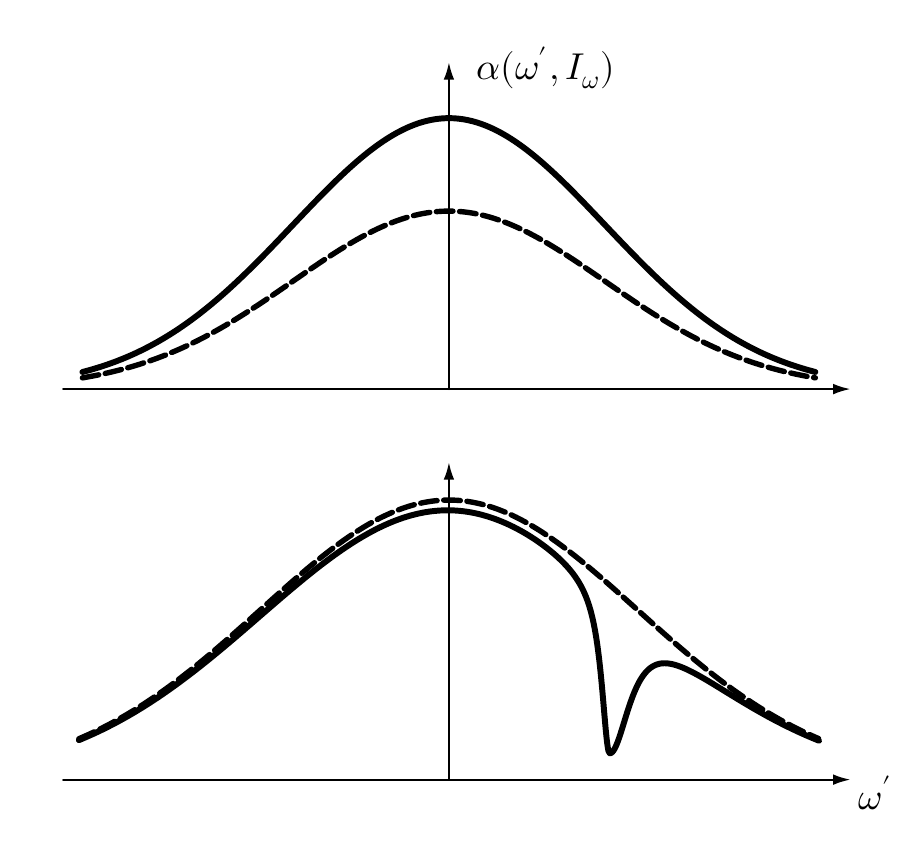
\begin{tikzpicture}[x=1cm,y=1cm,>=Latex,line cap=round,line join=round,font=\fontsize{15}{18}\selectfont]


% Upper panel: homogeneous saturation, lower: inhomogeneous hole-burning.
% Lower hole model: broad envelope × (1 - d/(1+((x-xr)/w_{L,R})²)).
% The piecewise tails make recovery on the right slower (source's shoulder).
\path[use as bounding box] (0,0) rectangle (10.9,10.3);
% Upper region
\begin{scope}[shift={(0,5.16)}]
 \draw[axis] (.45,.55)--(10.45,.55);
 \draw[axis] (5.35,.55)--(5.35,4.70);
 \node[smalllabel,anchor=west] at (5.58,4.63) {$\alpha(\omega',I_{\omega})$};
 \draw[curve,samples=410,domain=-4.75:4.75,smooth] plot ({5.35+.98*\x},{.55+3.44*exp(-(.35*\x)^2)});
 \draw[curveb,samples=410,domain=-4.75:4.75,smooth] plot ({5.35+.98*\x},{.55+2.26*exp(-(.35*\x)^2)});
\end{scope}
% Lower broad envelope and burn-out contour; the right shoulder is intentional.
\begin{scope}[shift={(0,.22)}]
 \draw[axis] (.45,.53)--(10.45,.53);
 \draw[axis] (5.35,.53)--(5.35,4.56);
 \node[smalllabel,anchor=west] at (10.43,.36) {$\omega'$};
 \draw[curveb,samples=400,domain=-4.7:4.7,smooth] plot ({5.35+1.0*\x},{.53+3.55*exp(-(.295*\x)^2)});
 \draw[curve,samples=560,domain=-4.7:4.7,smooth] plot ({5.35+1.0*\x},{.53+3.43*exp(-(.295*\x)^2)*(1-.86/(1+((\x-2.04)/(ifthenelse(\x<2.04,.12,.35)))^2))});
\end{scope}

\end{tikzpicture}
\end{document}
